\documentclass[conf]{new-aiaa}

\usepackage{amsmath,amssymb}
\usepackage{array}
\usepackage{multirow}
\usepackage{float}
\usepackage{graphicx}
\usepackage{geometry}

\usepackage{booktabs}
\usepackage{diagbox}
\usepackage[table,xcdraw]{xcolor}

\usepackage{siunitx}
\usepackage{longtable,tabularx}
\usepackage{caption}
\usepackage{subcaption}
\usepackage{hyperref}

\usepackage{minted}
\usemintedstyle{autumn}
\setminted{linenos,breaklines,tabsize=4,xleftmargin=1.5em}

\title{VE401 Term Project 2\\
Police Shootings in the United States}
\author{Group 21\\
Hongju Guang (516370910009),
Mingzhi Cai (517021911102),
Pengnan Chi (517370910245),\\
Xinyu Yan (517370910232) and
Yihao Liu (515370910207)
\footnote{Authors' names are in alphabet order.}
}
\affil{University OF Michigan - Shanghai Jiao Tong University Joint Institute, Shanghai, China}

\begin{document}

\maketitle

\begin{abstract}
In the article \textit{"London murders: a predictable pattern?"}, David Spiegelhalter and Arthur Barnett found that the London homicides follow a Poisson distribution. In this paper, we want to discuss the pattern of police shootings.

We want to test whether the occurrence of police shootings follows a Poisson distribution. We first estimate the parameter $k$ of Poisson distribution using the the occurrence of police shootings in the US in the years 2015-2018. We apply the test for goodness-of-fit to the police shootings in the three years and calculate the P-value. We conclude that the occurrence of police shootings follows a Poisson distribution with parameter $k\approx2.70$. We then test whether the average number of police shootings depends on the weekday using the Chi-squared test for independence. We also calculate the 95\% confidence interval for the parameter $k$ of the Poisson distribution. At last, we try to predict the occurrence of police shootings in 2019 and obtain 95\% prediction intervals for the number of mass shootings in 2019.

The method we use is very useful for pattern analyzing. We can first assume a likely distribution, and then estimate the parameter for the distribution, and then apply the goodness-of-fit test. After we conclude that the data follow the expected distribution, we can do some predictions.


    
\end{abstract}

\vspace{5cm}
\begin{center}
Keywords: Police shooting, Poisson distribution, Goodness-of-fit test, Test for independence.
\end{center}

\newpage

\tableofcontents
\newpage


\section{Nomenclature}

{\renewcommand\arraystretch{1.0}
\noindent\begin{longtable*}{@{}l @{\quad=\quad} l@{}}
$k$ & parameter of Poisson distribution \\
$\hat{k}$ & estimator of $k$ \\
$O_i$ & observed frequency \\
$E_i$ & expected frequency \\
$P[X=i]$ expected probability of category $i$ \\
$X^2$ & chi-squared distribution \\
$\chi^2_{\alpha,d}$ chi-squared distribution value of $d$ degrees of freedom at $\alpha$ level of significance \\
$Z$ standard normal distribution
\end{longtable*}}

\newpage

\section{Problem Statement}

\subsection{Introduction}

Fatal force and fatal shooting by police are topics that attract headlines and trigger heated debate around the world. When we are discussing these topics, it's important to have a clear image of what ``fatal police shooting'' is. Then we will discuss the pattern of police shootings regarding to the probability. 

According to the statistics from the Washington Post \cite{washingtonpost}, 962 people have been shot and killed by police in the US in 2016, and 994 people were fatally shot by police in 2015. The Washington Post is compiling such a database of every fatal shooting in the United States by a police officer in the line of duty since Jan. 1, 2015. This database is based on news reports, public records, social media and other sources.

For the term ``fatal police shooting,'' the Post characterizes it as those shootings in which a police officer, in the line of duty, shoots and kills a civilian — the circumstances that most closely parallel the 2014 killing of Michael Brown in Ferguson, Mo., which began the protest movement culminating in Black Lives Matter and attracted attention to police accountability nationwide \cite{questia}. What is worth attention is that the Post is not tracking deaths of people ``in police custody, fatal shootings by off-duty officers or non-shooting deaths.''

\begin{figure}[H]
	\centering
	\includegraphics[width=0.7\linewidth]{intro.png}  
	\caption{Silent protest for police shooting of Michael Brown.}  
\end{figure}

Of course every single murder is a tragedy for those whom it affects, but for the bettering of the police service and the benefit of broader society we may wish to consider whether these ``shocking'' numbers lead to some patterns. In the following content, we carry out a statistical analysis on the mass shootings in the US from 2015 - 2018, exploring the distribution pattern, the dependence on weekday and month, then anticipating the number of police shootings in 2019.

\subsection{Overview}

First, we use \emph{Mathematica} to visualize the fatal police shooting from the data provided by \emph{WashingtonPost}\cite{washingtonpost} between January 1$^{\rm st}$,2015 and December 31$^{\rm st}$, 2018. The plot was shown in Figure \ref{fig:q2}.

\begin{figure}[!htbp]
	\centering
	\includegraphics[width=0.9\linewidth]{q2/q2.eps}
	\caption{Number of fatal police shoots each day between January 1$^{\rm st}$,2015 and December 31$^{\rm st}$, 2018.}
	\label{fig:q2}
\end{figure}

Note that 2016 is a leap year, which means that there is one more day (February 29$^{\rm th}$) in 2016 than in the other three years, so the distance between 2016 and 2017 on the x-axis is slightly different from the distance between other years.

\subsection{Background}\ref{title:poisson}

We first introduce the Poisson distribution\cite{horst}.

Let $k\in \mathbb{R}$. A random variable $(X,f_{X})$ with $X:S\rightarrow \mathbb{N}$ and distribution function $f_{X}:\mathbb{N}\rightarrow\mathbb{R}$ given by
\begin{equation}
f_{X}(x)=\frac{k^xe^{-k}}{x!}
\end{equation}
is said to have a Poisson distribution with parameter $k$.\medskip

In fact the parameter $k$ of the Poisson distribution is also the expectation of the distribution.

\begin{equation}
E[X]=\sum_{x=0}^{\infty}x\frac{k^xe^{-k}}{x!}=\sum_{x=1}^{\infty}x\frac{k^xe^{-k}}{x!}=ke^{-k}\sum_{x-1=0}^{\infty}\frac{k^{x-1}}{(x-1)!}=ke^{-k}e^k=k
\end{equation}

We can use the property $E[x]=k$ to calculate the maximum-likelihood estimator of the parameter $k$.
\newpage

\section{Description of work}

\subsection{Distribution of fatal police shootings between 2015 and 2018}\label{title:q3}

In the work of Spiegelhalter and Barnett\cite{london}, the London homicides follow a Poisson distribution with parameter $k = 0.44$. We suggest that the distribution of fatal police shooting in the USA may be similar to that of London homicides, then we assume that the police shootings follow a Poisson distribution with an unknown parameter $k$ and perform a goodness-of-fit test for Poisson distribution.

\subsubsection{Hypothesis test of data in four years between 2015 and 2018}\label{title:q3-1}

First, we collect the fatal police shootings between 2015 and 2018 altogether and perform a hypothesis test. There are 1461 days in these four years, so that the random sample size is $n=1461$. We used \emph{Mathematica} to categorize and analyze the data according to the number of fatal police shootings $X$ and corresponding observed frequency $O_i$, as shown in Table \ref{tab:q3-all-obs} and Figure \ref{fig:q3-all-obs}. \medskip

\begin{table}[!htbp]
\centering
\begin{tabular}{m{3cm}<{\centering}m{3cm}<{\centering}}
\toprule 
\toprule
Number of fatal police shootings $X$    & Observed Frequency $O_i$ \\
\noalign{\smallskip}\hline\noalign{\smallskip}
0  &   108    \\
1  &   287   \\
2  &   324    \\
3  &   310    \\
4  &   227    \\
5  &   116    \\
6  &   53    \\
7  &   21    \\
8  &   11    \\
9  &   3    \\
10  &  1     \\
\bottomrule 
\bottomrule\smallskip
\end{tabular}
\caption{Observed Frequency $O_i$ versus each number of fatal police shootings data between 2015 and 2018.}
\label{tab:q3-all-obs}
\end{table}

\begin{figure}[!htbp]
\centering
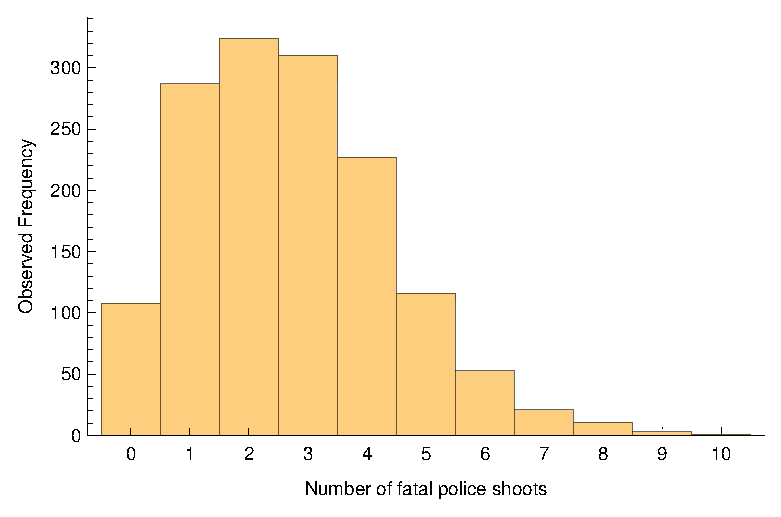
\includegraphics[height=7cm]{q3/q3-all-obs.eps}
\caption{Observed Frequency $O_i$ versus each number of fatal police shootings data between 2015 and 2018.}
\label{fig:q3-all-obs}
\end{figure}

The parameter $k$ of the assumed Poisson distribution is unknown and must be estimated from the data. According to \ref{title:poisson}, we know that a maximum-likelihood estimator for $k$ is the sample mean,
$$\hat{k} = \frac{1}{n}\sum_{i=0}^{10} X_iO_i = \frac{3943}{1461} \approx 2.70.$$
We test 
$$H_0:\text{the number of fatal police shootings follows a Poisson\ distribution with parameter }k = 2.70.$$

In order to transform the test of Poisson distribution into a test of categorical distribution, we first calculate the estimated probability for each category,
$$P[X=i]=\frac{e^{-\hat{k}}\hat{k}^i}{i!},\quad{\rm for\ }i\in[0,9],i\in Z,$$
and typically
$$P[X=10]=1-\sum_{i=0}^9P[X=i]=1-\sum_{i=0}^9\frac{e^{-\hat{k}}\hat{k}^i}{i!}$$
for the last category. The expected frequency can be calculated by
$$E_i=nP[X=i].$$
The calculated results were shown in Table \ref{tab:q3-all-exp}. \medskip

\begin{table}[!htbp]
\centering
\begin{tabular}{m{3cm}<{\centering}m{3cm}<{\centering}m{3cm}<{\centering}m{3cm}<{\centering}}
\toprule 
\toprule
Number of fatal police shootings $X$ (Category $i$)
 & Observed Frequency $O_i$ 
& Expected Probability $P[X=i]=\frac{e^{-\hat{k}}\hat{k}^i}{i!}$ & Expected Frequency $E_i=nP[X=i]$ \\
\noalign{\smallskip}\hline\noalign{\smallskip}
0  &   108   & 0.0673  & 98.30\\
1  &   287   & 0.1816   & 265.3\\
2  &   324   & 0.2450   & 358.0\\
3  &   310   & 0.2204   & 322.1\\
4  &   227   & 0.1487   & 217.3\\
5  &   116   & 0.0803  & 117.3\\
6  &   53    & 0.0361  & 52.76\\
7  &   21    & 0.0139  & 20.34\\
8  &   11    & 0.0047  & 6.862\\
9  &   3     & 0.0014 & 2.058\\
$\geqslant$10 &   1     & $4.997\times10^{-4}$& 0.730\\\hline
$\geqslant$9 &   4     & 0.0019& 2.788\\
\bottomrule 
\bottomrule  \smallskip
\end{tabular}
\caption{Expected probability and frequency for the categorized fatal police shootings data between 2015 and 2018.}
\label{tab:q3-all-exp}
\end{table}

According to the Pearson Statistic, two generally stated criteria of  categorical distribution are
\begin{align}
E_i=nP[X=i]\geqslant1 & \qquad {\rm for\ all\ }i=1,\dots,N,\\
E_i=nP[X=i]\geqslant5 & \qquad {\rm for\ 80\%\ of\ all\ }i=1,\dots,N,
\end{align}
where $N$ is the number of the categories. In our data, we can find that $E_{10}=0.730095<1$, which doesn't satisfy the criteria. The problem can be solved by combining the last two categories, which makes
\begin{align*}
&O_9'=O_9+O_{10}=4,\\
&P[X\geqslant9]=P[X=9]+P[X\geqslant10]\approx 0.0019,\\
&E_9'=nP[X\geqslant9]\approx2.788.
\end{align*}
Now only one category has an expectation less than 5, and all of the categories have expectations greater then 1, which satisfies the criteria. The origin test is then equivalent to the test
$$H_0:\text{the number of fatal police shootings follows a categorical distribution with parameters }\{E_i\}.$$

For $N = 10$ categories, the statistic
\begin{equation}
X^2=\sum_{i=0}^{N-1}\frac{(O_i-E_i)^2}{E_i}
\end{equation}
then follows a chi-squared distribution with $N-1-m=10-1-1=8$
degree of freedom, where $m$ is the number of estimated parameters. With the data, we have
$$X^2\approx9.9049,$$
and we can reject $H_0$ at $\alpha$ level of significance if $X^2>\chi^2_{\alpha,8}$. When $\alpha\approx0.448876$,
$$\chi^2_{\alpha,8}\approx9.9049=X^2,$$
so the P-value of the test is $0.448876$, which is much larger than 0.05. \medskip

We also plotted Figure \ref{fig:q3-all-exp} to show the observed frequency $O_i$, expected Frequency $E_i$ and estimated Poisson distribution. The data fit the curve fine, which also gives evidence that it follow a Poisson distribution. \medskip

\begin{figure}[!htbp]
\centering
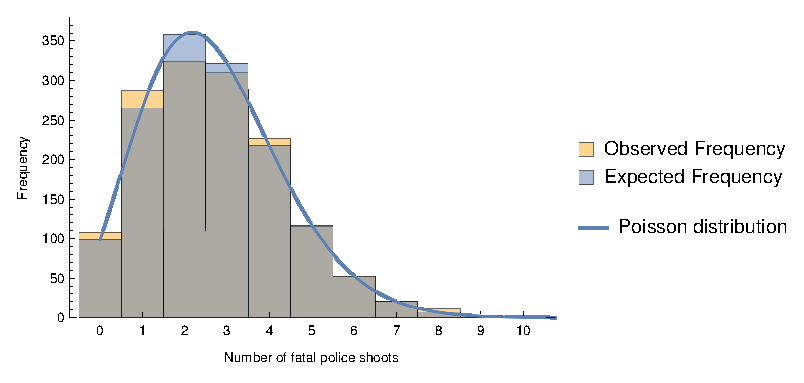
\includegraphics[height=7cm]{q3/q3-all-exp.eps}
\caption{Observed Frequency $O_i$, Expected Frequency $E_i$ and estimated Poisson distribution versus each number of fatal police shootings data between 2015 and 2018.}
\label{fig:q3-all-exp}
\end{figure}

In conclusion, we have no evidence to reject $H_0$ at 5\% level of significance, which means the fatal police shootings between 2015 and 2018 is likely to follow a Poisson distribution with $k=2.70.$

\subsubsection{Hypothesis test of data in individual years}

Although the Hypothesis test for all years showed that the overall data follow a Poisson distribution, we were also curious about the circumstance in individual years. \medskip

The procedure of the hypothesis test of Poisson distribution in the individual years is exactly the same as that for all years (\ref{title:q3-1}), we will omit some detailed deduction and provide the results for each year individually.

\paragraph{Year 2015}\ 

The categorized data, expected probability and frequency were shown in Table \ref{tab:q3-2015-exp}. \medskip

\begin{table}[!htbp]
\centering
\begin{tabular}{m{3cm}<{\centering}m{3cm}<{\centering}m{3cm}<{\centering}m{3cm}<{\centering}}
\toprule 
\toprule
Number of fatal police shootings $X$ (Category $i$)
 & Observed Frequency $O_i$ 
& Expected Probability $P[X=i]$ & Expected Frequency $E_i$ \\
\noalign{\smallskip}\hline\noalign{\smallskip}
0  &   24   & 0.0655  & 23.90\\
1  &   73   & 0.1785   & 65.15\\
2  &   87   & 0.2433   & 88.80\\
3  &   69   & 0.2211   & 80.69\\
4  &   55   & 0.1507   & 54.99\\
5  &   33   & 0.0821  & 29.98\\
6  &   14   & 0.0373  & 13.62\\
7  &   8    & 0.0145  & 5.305\\
$\geqslant$8  &   2    & 0.0070  & 2.552\\\hline
$\geqslant$7  &   10    & 0.0215  & 7.857\\
\bottomrule 
\bottomrule  \smallskip
\end{tabular}
\caption{Expected probability and frequency for the categorized fatal police shootings data in 2015.}
\label{tab:q3-2015-exp}
\end{table}

Here we have
\begin{align*}
&n=365,\\
&\hat{k} = \frac{1}{n}\sum_{i=0}^{8} X_iO_i = \frac{199}{73} \approx 2.73,\\
&O_7'=O_7+O_8=10,\\
&P[X\geqslant7]=P[X=7]+P[X\geqslant8]\approx 0.0215,\\
&E_7'=nP[X\geqslant7]\approx7.857,\\
&X^2=\sum_{i=0}^{N-1}\frac{(O_i-E_i)^2}{E_i}\approx3.5756,\\
&\text{P-value}\approx0.8932.
\end{align*}

The P-value of the test is is much larger than 0.05, and the data fit the curve fine in Figure \ref{fig:q3-2015-exp}. We can claim that the fatal police shootings in 2015 and is likely to follow a Poisson distribution with $k=2.73$ at 5\% level of significance.

\begin{figure}[!htbp]
\centering
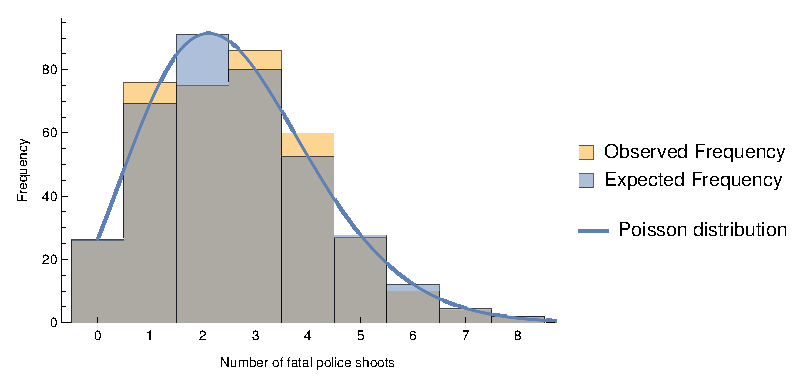
\includegraphics[height=7cm]{q3/q3-2015-exp.eps}
\caption{Observed Frequency $O_i$, Expected Frequency $E_i$ and estimated Poisson distribution versus each number of fatal police shootings data in 2015.}
\label{fig:q3-2015-exp}
\end{figure}

\paragraph{Year 2016}\ 

The categorized data, expected probability and frequency were shown in Table \ref{tab:q3-2016-exp}. \medskip

\begin{table}[!htbp]
\centering
\begin{tabular}{m{3cm}<{\centering}m{3cm}<{\centering}m{3cm}<{\centering}m{3cm}<{\centering}}
\toprule 
\toprule
Number of fatal police shootings $X$ (Category $i$)
 & Observed Frequency $O_i$ 
& Expected Probability $P[X=i]$ & Expected Frequency $E_i$ \\
\noalign{\smallskip}\hline\noalign{\smallskip}
0  &   26   & 0.0720  & 26.35\\
1  &   76   & 0.1894   & 69.33\\
2  &   75   & 0.2492   & 91.21\\
3  &   86   & 0.2186   & 80.00\\
4  &   60   & 0.1438   & 52.62\\
5  &   27   & 0.0757   & 27.69\\
6  &   10   & 0.0331   & 12.14\\
7  &   4    & 0.0125   & 4.564\\
$\geqslant$8  &   2    & $5.712\times10^{-4}$  & 2.091\\
\bottomrule 
\bottomrule  \smallskip
\end{tabular}
\caption{Expected probability and frequency for the categorized fatal police shootings data in 2016.}
\label{tab:q3-2016-exp}
\end{table}

Here we have
\begin{align*}
&n=366,\\
&\hat{k} = \frac{1}{n}\sum_{i=0}^{8} X_iO_i = \frac{321}{122} \approx 2.63,\\
&X^2=\sum_{i=0}^{N-1}\frac{(O_i-E_i)^2}{E_i}\approx5.4817,\\
&\text{P-value}\approx0.7905.
\end{align*}

The P-value of the test is is much larger than 0.05, and the data fit the curve fine in Figure \ref{fig:q3-2016-exp}. We can claim that the fatal police shootings in 2016 and is likely to follow a Poisson distribution with $k=2.63$ at 5\% level of significance.

\begin{figure}[!htbp]
\centering
\includegraphics[height=7cm]{q3/q3-2016-exp.eps}
\caption{Observed Frequency $O_i$, Expected Frequency $E_i$ and estimated Poisson distribution versus each number of fatal police shootings data in 2016.}
\label{fig:q3-2016-exp}
\end{figure}

\paragraph{Year 2017}\ 

The categorized data, expected probability and frequency were shown in Table \ref{tab:q3-2017-exp}. \medskip

\begin{table}[!htbp]
\centering
\begin{tabular}{m{3cm}<{\centering}m{3cm}<{\centering}m{3cm}<{\centering}m{3cm}<{\centering}}
\toprule 
\toprule
Number of fatal police shootings $X$ (Category $i$)
 & Observed Frequency $O_i$ 
& Expected Probability $P[X=i]$ & Expected Frequency $E_i$ \\
\noalign{\smallskip}\hline\noalign{\smallskip}
0  &   23   & 0.0670   & 24.43\\
1  &   67   & 0.1810   & 66.06\\
2  &   86   & 0.2447   & 89.32\\
3  &   87   & 0.2206   & 80.51\\
4  &   53   & 0.1491   & 54.43\\
5  &   28   & 0.0806   & 29.43\\
6  &   16   & 0.0363   & 13.27\\
7  &   1    & 0.0140   & 5.125\\
$\geqslant$8  &   4    & $6.679\times10^{-4}$  & 2.438\\
\bottomrule 
\bottomrule  \smallskip
\end{tabular}
\caption{Expected probability and frequency for the categorized fatal police shootings data in 2017.}
\label{tab:q3-2017-exp}
\end{table}

Here we have
\begin{align*}
&n=365,\\
&\hat{k} = \frac{1}{n}\sum_{i=0}^{8} X_iO_i = \frac{987}{365} \approx 2.70,\\
&X^2=\sum_{i=0}^{N-1}\frac{(O_i-E_i)^2}{E_i}\approx5.7355,\\
&\text{P-value}\approx0.7661.
\end{align*}

The P-value of the test is is much larger than 0.05, and the data fit the curve fine in Figure \ref{fig:q3-2017-exp}. We can claim that the fatal police shootings in 2017 and is likely to follow a Poisson distribution with $k=2.70$ at 5\% level of significance.

\begin{figure}[!htbp]
\centering
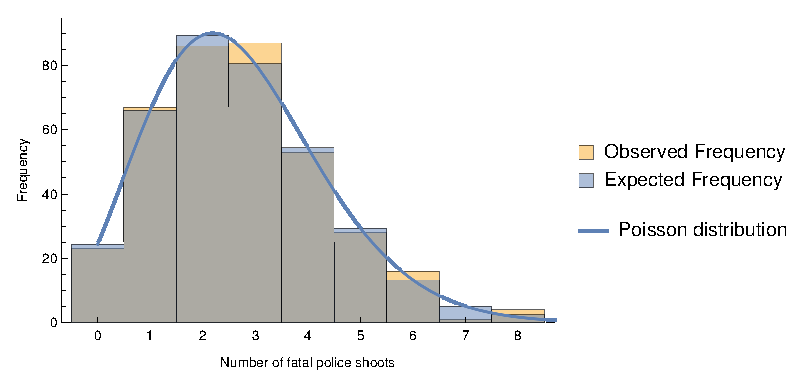
\includegraphics[height=7cm]{q3/q3-2017-exp.eps}
\caption{Observed Frequency $O_i$, Expected Frequency $E_i$ and estimated Poisson distribution versus each number of fatal police shootings data in 2017.}
\label{fig:q3-2017-exp}
\end{figure}

\paragraph{Year 2018}\ 

The categorized data, expected probability and frequency were shown in Table \ref{tab:q3-2018-exp}. \medskip

\begin{table}[!htbp]
\centering
\begin{tabular}{m{3cm}<{\centering}m{3cm}<{\centering}m{3cm}<{\centering}m{3cm}<{\centering}}
\toprule 
\toprule
Number of fatal police shootings $X$ (Category $i$)
 & Observed Frequency $O_i$ 
& Expected Probability $P[X=i]$ & Expected Frequency $E_i$ \\
\noalign{\smallskip}\hline\noalign{\smallskip}
0  &   35   & 0.0649  & 23.70\\
1  &   71   & 0.1776   & 64.81\\
2  &   76   & 0.2428   & 88.61\\
3  &   68   & 0.2213   & 80.76\\
4  &   59   & 0.1512   & 55.20\\
5  &   28   & 0.0827  & 30.19\\
6  &   13   & 0.0377  & 13.76\\
7  &   8    & 0.0147  & 5.374\\
8  &   3    & 0.0050  & 1.837\\
9  &   3    & 0.0015  & 0.558\\
$\geqslant$10  &   1    & $5.517\times10^{-4}$  & 0.201\\\hline
$\geqslant$8  &   7    & 0.0071  & 2.596\\
\bottomrule 
\bottomrule  \smallskip
\end{tabular}
\caption{Expected probability and frequency for the categorized fatal police shootings data in 2018.}
\label{tab:q3-2018-exp}
\end{table}

Here we have
\begin{align*}
&n=365,\\
&\hat{k} = \frac{1}{n}\sum_{i=0}^{10} X_iO_i = \frac{998}{365} \approx 2.73,\\
&O_8'=O_8+O_9+O_{10}=7,\\
&P[X\geqslant8]=P[X=8]+P[X\geqslant9]+P[X\geqslant10]\approx 0.0071,\\
&E_8'=nP[X\geqslant8]\approx2.596,\\
&X^2=\sum_{i=0}^{N-1}\frac{(O_i-E_i)^2}{E_i}\approx19.000,\\
&\text{P-value}\approx0.025.
\end{align*}

The P-value of the test is is smaller than 0.05, and the data don't fit the curve fine in Figure \ref{fig:q3-2018-exp}. We can claim that the fatal police shootings in 2018 and is not likely to follow a Poisson distribution at 5\% level of significance.

\begin{figure}[!htbp]
\centering
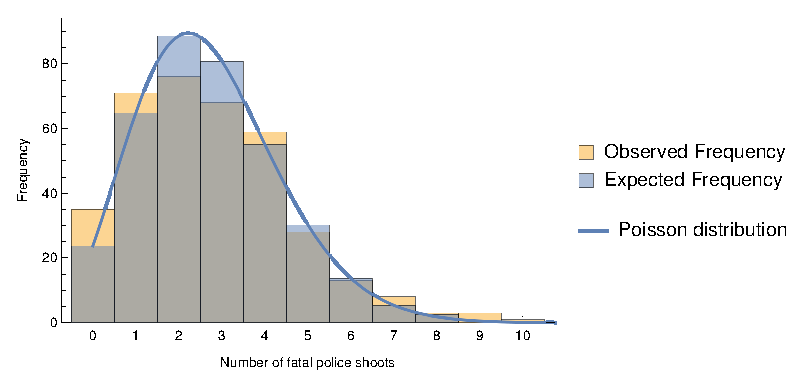
\includegraphics[height=7cm]{q3/q3-2018-exp.eps}
\caption{Observed Frequency $O_i$, Expected Frequency $E_i$ and estimated Poisson distribution versus each number of fatal police shootings data in 2018.}
\label{fig:q3-2018-exp}
\end{figure}

\newpage

\subsection{Independence test of fatal police shootings}

We also performed some independence tests with the data of fatal police shootings. We studied it in two extents: the relationship between average number of police shootings and weekdays or months, and the relationship between years and weekdays or months.

\subsubsection{Hypothesis test of data by average number of police shootings and weekdays}

First, we created a histogram with the data between 2015 and 2018, sorted by weekdays, as shown in Figure \ref{fig:q4-day}. \medskip

\begin{figure}[!htbp]
\centering
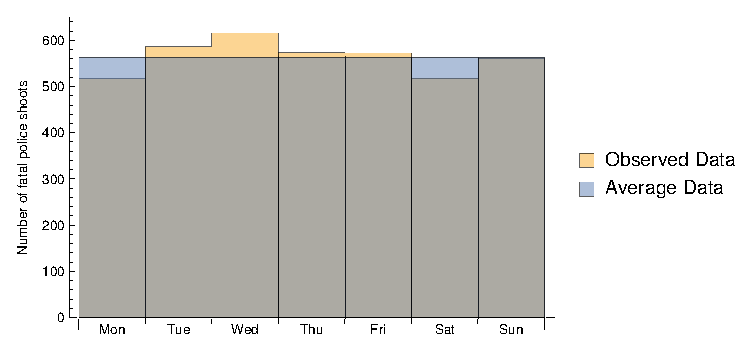
\includegraphics[height=7cm]{q4/q4-day.eps}
\caption{Number of fatal police shootings in each weekday between 2015 and 2018.}
\label{fig:q4-day}
\end{figure}

We test
$$H_0: \text{The data follow a multinomial distribution with same parameters }p=\frac{1}{7}.$$

The categorized data were shown in Table \ref{tab:q4-day}, where $E_i$ is the average number of police shootings in each weekday between 2015 and 2018. \medskip

\begin{table}[!htbp]
\centering
\begin{tabular}{c|ccccccc|c}
\toprule 
\toprule
 & Mon & Tue & Wed & Thu & Fri & Sat & Sun & Total \\
\hline
$O_i$ & 517 & 586 & 616 & 573 & 572 & 518 & 561 & \multirow{2}{*}{3943}\\
$E_i$ & 563.286 & 563.286 & 563.286 & 563.286 & 563.286 & 563.286 & 563.286 & \\
\bottomrule 
\bottomrule\noalign{\bigskip}
\end{tabular}
\caption{Observed Frequency $O_i$ and Expected Frequency $E_i$ of fatal police shootings in each weekday between 2015 and 2018.}
\label{tab:q4-day}
\end{table}

For $N=7$ categories, the statistic
\begin{equation}
X^2=\sum_{i=1}^N\frac{(O_i-E_i)^2}{E_i}
\end{equation}
then follows a chi-squared distribution with $N-1=6$ degree of freedom. With the data, we have
$$X^2\approx13.605,$$
and we can reject $H_0$ at $\alpha$ level of significance if $X^2>\chi^2_{\alpha,6}$. When $\alpha\approx0.0343753$,
$$\chi^2_{\alpha,6}\approx13.605=X^2,$$
so the P-value of the test is 0.0343753, which is smaller than 0.05. \medskip

Then $H_0$ is rejected at 5\% level of significance. However the P-value  is not small enough, i.e., we can not reject $H_0$ is rejected at 2.5\% level of significance, so we decided to apply the same test to different years in order to receive a further conclusion. \medskip

We created histograms with the data of each individual year, sorted by weekdays, as shown in Figure \ref{fig:q4-day-individual}. \medskip

\begin{figure}[!htbp]
\centering
\begin{subfigure}{.49\textwidth}
  \centering
  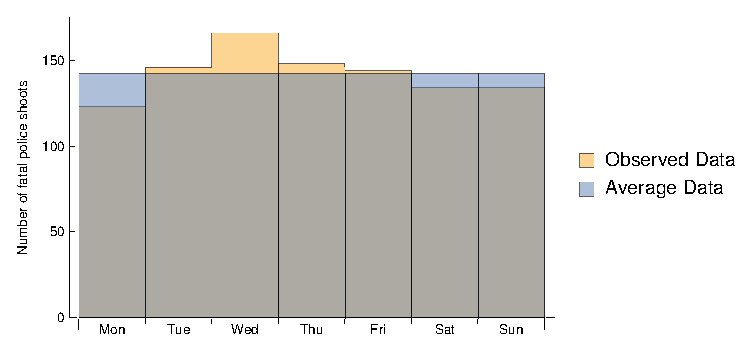
\includegraphics[width=\linewidth]{q4/q4-day-2015.eps}  
  \caption{Year 2015.}
  \label{fig:q4-day-2015}
\end{subfigure}
\begin{subfigure}{.49\textwidth}
  \centering
  \includegraphics[width=\linewidth]{q4/q4-day-2016.eps}  
  \caption{Year 2016.}
  \label{fig:q4-day-2016}
\end{subfigure}
\begin{subfigure}{.49\textwidth}
  \centering
  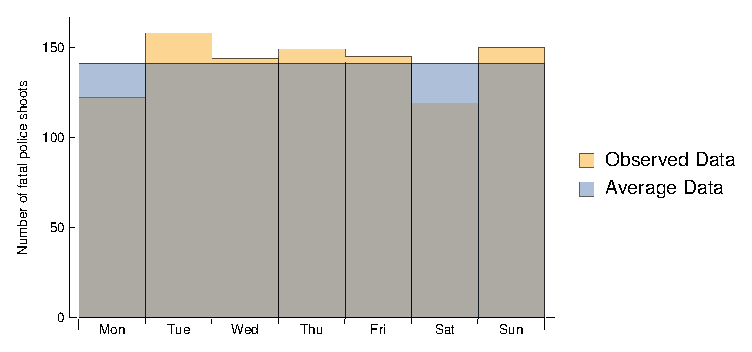
\includegraphics[width=\linewidth]{q4/q4-day-2017.eps}  
  \caption{Year 2017.}
  \label{fig:q4-day-2017}
\end{subfigure}
\begin{subfigure}{.49\textwidth}
  \centering
  \includegraphics[width=\linewidth]{q4/q4-day-2018.eps}  
  \caption{Year 2018.}
  \label{fig:q4-day-2018}
\end{subfigure}
\caption{Number of fatal police shootings in each weekday for each individual year between 2015 and 2018.}
\label{fig:q4-day-individual}
\end{figure}

The categorized data, calculated $X^2$ statistics and P-values were shown in Table \ref{tab:q4-day-individual}. We can find that all of the P-values are greater then 0.05, thus there is no evidence to reject $H_0$ for each individual year at 5\% level of significance. \medskip

\begin{table}[!htbp]
\centering
\begin{tabular}{cc|ccccccc|cc}
\toprule 
\toprule
\multicolumn{2}{c|}{Year} & Mon & Tue & Wed & Thu & Fri & Sat & Sun & $X^2$ & P-value\\
\hline
\multirow{2}{*}{2015} & $O_i$ & 123 & 146 & 166 & 148 & 144 & 134 & 134 & \multirow{2}{*}{7.885} & \multirow{2}{*}{0.247}\\
& $E_i$ & 142.143 & 142.143 & 142.143 & 142.143 & 142.143 & 142.143 & 142.143 & \\
\hline
\multirow{2}{*}{2016} & $O_i$ & 126 & 148 & 141 & 137 & 133 & 135 & 143 & \multirow{2}{*}{2.266} & \multirow{2}{*}{0.894}\\
& $E_i$ & 137.571 & 137.571 & 137.571 & 137.571 & 137.571 & 137.571 & 137.571 & \\
\hline
\multirow{2}{*}{2017} & $O_i$ & 122 & 158 & 144 & 149 & 145 & 119 & 150 & \multirow{2}{*}{9.248} & \multirow{2}{*}{0.160}\\
& $E_i$ & 141 & 141 & 141 & 141 & 141 & 141 & 141 & \\
\hline
\multirow{2}{*}{2018} & $O_i$ & 146 & 134 & 165 & 139 & 150 & 130 & 134 & \multirow{2}{*}{6.226} & \multirow{2}{*}{0.398}\\
& $E_i$ & 142.571 & 142.571 & 142.571 & 142.571 & 142.571 & 142.571 & 142.571 & \\
\bottomrule 
\bottomrule\noalign{\bigskip}
\end{tabular}
\caption{Observed Frequency $O_i$, Expected Frequency $E_i$, $X^2$ statistic and P-value of fatal police shootings in each weekday for each individual year between 2015 and 2018.}
\label{tab:q4-day-individual}
\end{table}

In conclusion, there is no strong evidence that the
average number of police shootings depends on the weekday.

\subsubsection{Hypothesis test of data by average number of police shootings and months}

We also tested the relationship between average number of police shootings and months. The method of the test is exactly the same as shown in the previous part. The histograms were shown in Figure \ref{fig:q4-month} and the categorized data, calculated $X^2$ statistics and P-values were shown in Table \ref{tab:q4-month}. \medskip

\begin{figure}[!htbp]
\centering
\begin{subfigure}{.75\textwidth}
  \centering
  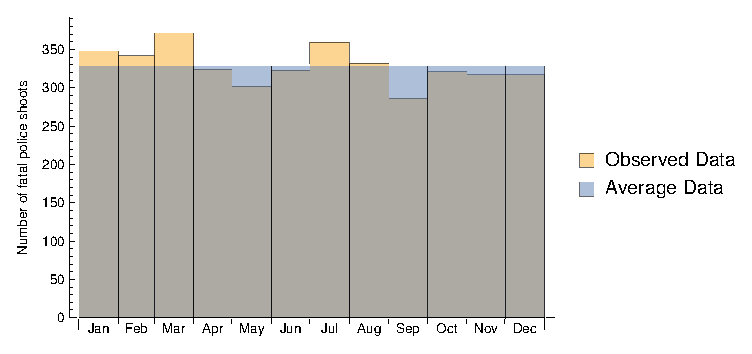
\includegraphics[width=\linewidth]{q4/q4-month.eps}  
  \caption{Overall.}
  \label{fig:q4-month-overall}
\end{subfigure}
\begin{subfigure}{.49\textwidth}
  \centering
  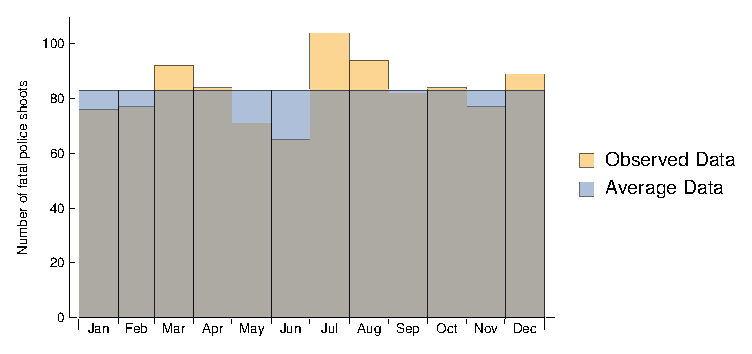
\includegraphics[width=\linewidth]{q4/q4-month-2015.eps}  
  \caption{Year 2015.}
  \label{fig:q4-month-2015}
\end{subfigure}
\begin{subfigure}{.49\textwidth}
  \centering
  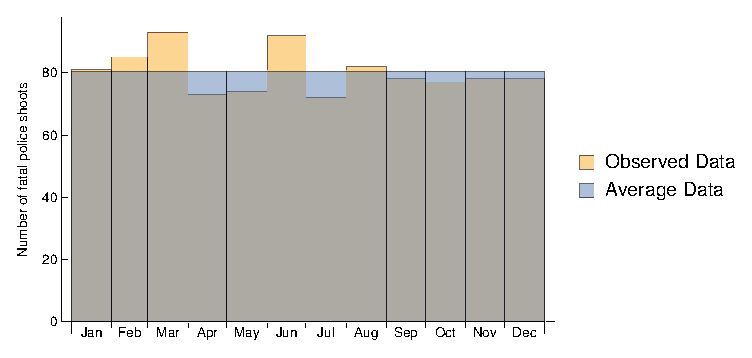
\includegraphics[width=\linewidth]{q4/q4-month-2016.eps}  
  \caption{Year 2016.}
  \label{fig:q4-month-2016}
\end{subfigure}
\begin{subfigure}{.49\textwidth}
  \centering
  \includegraphics[width=\linewidth]{q4/q4-month-2017.eps}  
  \caption{Year 2017.}
  \label{fig:q4-month-2017}
\end{subfigure}
\begin{subfigure}{.49\textwidth}
  \centering
  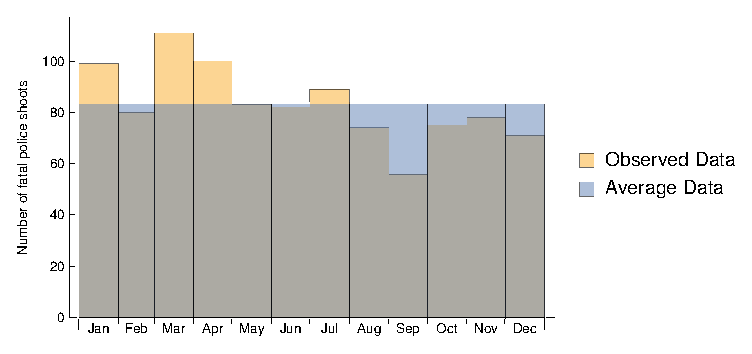
\includegraphics[width=\linewidth]{q4/q4-month-2018.eps}  
  \caption{Year 2018.}
  \label{fig:q4-month-2018}
\end{subfigure}
\caption{Number of fatal police shootings in each month between 2015 and 2018.}
\label{fig:q4-month}
\end{figure}

\begin{table}[!htbp]
\centering
\begin{tabular}{cc|cccccccccccc|cc}
\toprule 
\toprule
\multicolumn{2}{c|}{Year} & Jan & Feb & Mar & Apr & May & Jun & Jul & Aug & Sep & Oct & Nov & Dec & $X^2$ & P-value\\
\hline
\multirow{2}{*}{Total} & $O_i$ & 348 & 343 & 371 & 324 & 302 & 323 & 359 & 332 & 286 & 321 & 317 & 317 & \multirow{2}{*}{44.087} & \multirow{2}{*}{0.094}\\
& $E_i$ &&&&&&\multicolumn{2}{c}{328.583}&&&&&& \\
\hline
\multirow{2}{*}{2015} & $O_i$ & 76 & 77 & 92 & 84 & 71 & 65 & 104 & 94 & 82 & 84 & 77 & 89 & \multirow{2}{*}{15.328} & \multirow{2}{*}{0.168}\\
& $E_i$ &&&&&&\multicolumn{2}{c}{82.917}&&&&&& \\
\hline
\multirow{2}{*}{2016} & $O_i$ & 81 & 86 & 92 & 73 & 74 & 92 & 72 & 82 & 78 & 77 & 78 & 78 & \multirow{2}{*}{6.209} & \multirow{2}{*}{0.859}\\
& $E_i$ &&&&&&\multicolumn{2}{c}{80.25}&&&&&& \\
\hline
\multirow{2}{*}{2017} & $O_i$ & 92 & 100 & 76 & 67 & 74 & 84 & 94 & 82 & 70 & 85 & 84 & 79 & \multirow{2}{*}{12.915} & \multirow{2}{*}{0.299}\\
& $E_i$ &&&&&&\multicolumn{2}{c}{82.25}&&&&&& \\
\hline
\multirow{2}{*}{2018} & $O_i$ & 99 & 80 & 111 & 100 & 83 & 82 & 89 & 74 & 56 & 75 & 78 & 71 & \multirow{2}{*}{29.070} & \multirow{2}{*}{0.0022}\\
& $E_i$ &&&&&&\multicolumn{2}{c}{83.167}&&&&&& \\
\bottomrule 
\bottomrule\noalign{\bigskip}
\end{tabular}
\caption{Observed Frequency $O_i$, Expected Frequency $E_i$, $X^2$ statistic and P-value of fatal police shootings in each month between 2015 and 2018.}
\label{tab:q4-month}
\end{table}

We can find that except in year 2018, the overall data and the data for each year between 2015 and 2017 have a P-value greater than 0.05. In the figure we can not find any apparent evidence of the relationship between  average number of police shootings and months. However, the results for 2018 in quite interesting, we noticed a rising in March and April and a decay in September. We guessed that it may be related to some government policies in that year, and more investigation of this part can be done with the future data in 2019. \medskip

In conclusion, there is no strong evidence that the
average number of police shootings depends on the month.

\subsubsection{Hypothesis test of data by years and weekdays}

We also tested the relationship between the years and weekdays with independence test. The data were shown in Table \ref{tab:q4-year-day-obs}.

\begin{table}[!htbp]
\centering
\begin{tabular}{c|ccccccc|c}
\toprule 
\toprule
Year & Mon & Tue & Wed & Thu & Fri & Sat & Sun & Total \\
\hline
2015 & 123 & 146 & 166 & 148 & 144 & 134 & 134 & 995\\
2016 & 126 & 148 & 141 & 137 & 133 & 135 & 143 & 963\\
2017 & 122 & 158 & 144 & 149 & 145 & 119 & 150 & 987\\
2018 & 146 & 134 & 165 & 139 & 150 & 130 & 134 & 998\\
\hline
Total & 517 & 586 & 616 & 573 & 572 & 518 & 561 & 3943\\
\bottomrule 
\bottomrule\noalign{\bigskip}
\end{tabular}
\caption{Observed Frequency $O_{i,j}$ categorized by years and weekdays of fatal police shootings data between 2015 and 2018.}
\label{tab:q4-year-day-obs}
\end{table}

Then we can calculate the expectation by
$$E_{ij}=\frac{n_in_j}{n}.$$

The results were shown in Table \ref{tab:q4-year-day-exp}.

\begin{table}[!htbp]
\centering
\begin{tabular}{c|ccccccc}
\toprule 
\toprule
Year & Mon & Tue & Wed & Thu & Fri & Sat & Sun  \\
\hline
2015 & 130.463 & 147.875 & 155.445 & 144.594 & 144.342 & 130.715 & 141.566 \\
2016 & 126.267 & 143.119 & 150.446 & 139.944 & 139.7 & 126.511 & 137.013 \\
2017 & 129.414 & 146.686 & 154.195 & 143.432 & 143.181 & 129.664 & 140.428 \\
2018 & 130.856 & 148.321 & 155.914 & 145.03 & 144.777 & 131.109 & 141.993 \\
\bottomrule 
\bottomrule\noalign{\bigskip}
\end{tabular}
\caption{Expected Frequency $E_{i,j}$ categorized by years and weekdays of fatal police shootings data between 2015 and 2018.}
\label{tab:q4-year-day-exp}
\end{table}

It is now a simple matter to calculate the value of the statistic
$$X^2_{r-1,c-1}=\sum_{i=1}^r\sum_{j=1}^c\frac{(O_{ij}-E_{ij})^2}{E_{ij}},$$
where $r$ and $c$ are the column and row numbers. \medskip

The degree of freedom of this test is $3\times6=18$, we get $X^2\approx12.013$ and the P-value of the test is $0.847$. There is no evidence that there is relationship between years and weekdays. 

\subsubsection{Hypothesis test of data by years and months}

We also tested the relationship between the years and weekdays with independence test. The data were shown in Table \ref{tab:q4-year-month-obs}.

\begin{table}[!htbp]
\centering
\begin{tabular}{c|cccccccccccc|c}
\toprule 
\toprule
Year & Jan & Feb & Mar & Apr & May & Jun & Jul & Aug & Sep & Oct & Nov & Dec & Total \\
\hline
2015 & 76 & 77 & 92 & 84 & 71 & 65 & 104 & 94 & 82 & 84 & 77 & 89 & 995\\
2016 & 81 & 86 & 92 & 73 & 74 & 92 & 72 & 82 & 78 & 77 & 78 & 78 & 963\\
2017 & 92 & 100 & 76 & 67 & 74 & 84 & 94 & 82 & 70 & 85 & 84 & 79 & 987\\
2018 & 99 & 80 & 111 & 100 & 83 & 82 & 89 & 74 & 56 & 75 & 78 & 71 & 998\\
\hline
Total & 348 & 343 & 371 & 324 & 302 & 323 & 359 & 332 & 286 & 321 & 317 & 317 & 3943\\
\bottomrule 
\bottomrule\noalign{\bigskip}
\end{tabular}
\caption{Observed Frequency $O_{i,j}$ categorized by years and months of fatal police shootings data between 2015 and 2018.}
\label{tab:q4-year-month-obs}
\end{table}

Then we can calculate the expectation by
$$E_{ij}=\frac{n_in_j}{n}.$$

The results were shown in Table \ref{tab:q4-year-month-exp}.

\begin{table}[!htbp]
\centering
\begin{tabular}{c|cccccccccccc}
\toprule 
\toprule
Year & Jan & Feb & Mar & Apr & May & Jun & Jul & Aug & Sep & Oct & Nov & Dec \\
\hline
2015 & 87.81 & 86.55 & 93.62 & 81.76 & 76.20 & 81.50 & 90.59 & 83.77 & 72.17 & 81.00 & 79.99 & 79.99 \\
2016 & 84.99 & 83.77 & 90.60 & 79.13 & 73.75 & 78.88 & 87.67 & 81.08 & 69.84 & 78.39 & 77.42 & 77.42 \\
2017 & 87.11 & 85.85 & 92.86 & 81.10 & 75.59 & 80.85 & 89.86 & 83.10 & 71.59 & 80.35 & 79.35 & 79.35 \\
2018 & 88.08 & 86.81 & 93.90 & 82.00 & 76.43 & 81.75 & 90.86 & 84.03 & 72.38 & 81.24 & 80.23 & 80.23 \\
\bottomrule 
\bottomrule\noalign{\bigskip}
\end{tabular}
\caption{Expected Frequency $E_{i,j}$ categorized by years and months of fatal police shootings data between 2015 and 2018.}
\label{tab:q4-year-month-exp}
\end{table}

It is now a simple matter to calculate the value of the statistic
$$X^2_{r-1,c-1}=\sum_{i=1}^r\sum_{j=1}^c\frac{(O_{ij}-E_{ij})^2}{E_{ij}},$$
where $r$ and $c$ are the column and row numbers. \medskip

The degree of freedom of this test is $3\times11=33$, we get $X^2\approx44.087$ and the P-value of the test is $0.094$. There is no evidence that there is relationship between years and months.



\subsection{Confidence intervals of the distribution}

Let the random variable $X$ denote the everyday occurrence of police shooting in the United States. We have verified that $X$ follows a Poisson distribution, $$p(x)=\frac{(k)^{x}}{x !} e^{k}.$$ 
Now we are of interest in the confidence interval for the parameter $k$we obtained in section \ref{title:q3}.

\subsubsection{The formula of confidence interval}

We have already known that the a maximum-likelihood estimator for $k$ is the sample mean, $\overline{X}$. \medskip

Since our sample size is sufficient large, with the central limit theorem, it is advisable to say that our sample mean follows a normal distribution. Furthermore, we have a standard normal distribution
\begin{equation}\label{eq:std}
    Z=\frac{\overline{X}-k}{\sigma / \sqrt{n}}. 
\end{equation}

We then need to find and estimator for the variance $\sigma^2$. With the property Poisson distribution. The variance of $X$ should be $\text{Var }X = k$. Therefore, the estimator for variance is the estimator for k, which is the sample mean, $\overline{X}$. Now we rewrite Eq. \ref{eq:std} as 
\begin{equation}
Z = \frac{\hat{k}-k}{ \hat{k}/ \sqrt{n}},
\end{equation}
where $\hat{k}$ is the estimator for $k$, which is $\overline{X}$.\medskip

According to Theorem 2.2.16\cite{horst}, a $(1 - \alpha)100\%$
confidence interval on the sample mean $\mu$ of a normal distribution is given by 
\begin{equation}\label{eq:ci}
\overline{X}\pm\frac{z_{\alpha/2}\cdot\sigma}{\sqrt{n}}.
\end{equation}

Rewrite the formula we get the $(1 - \alpha)100\%$
confidence interval for $k$,
\begin{equation}
\hat{k} \pm z_{\alpha / 2} \sqrt{\hat{k} / n}.
\end{equation}

\subsubsection{Confidence intervals of the parameters in Poisson distributions of fatal police shootings}

With the formula, we can calculate the 95\% confidence intervals with
$$z_{\alpha/2}=z_{0.025}\approx1.96.$$

The results were shown in Table \ref{tab:q5}.\medskip

\begin{table}[!htbp]
\centering
\begin{tabular}{ccccc}
\toprule 
\toprule
Year & Days & $n$ & $\hat{k}$ & 95\% confidence interval of $\hat{k}$ \\
\hline
All & 1461 & 3943 & 2.70 & $(2.65,2.75)$\\
2015 & 365 & 995  & 2.73 & $(2.62,2.83)$\\
2016 & 366 & 963  & 2.63 & $(2.53,2.73)$\\
2017 & 365 & 987  & 2.70 & $(2.60,2.81)$\\
2018 & 365 & 998  & 2.73 & $(2.63,2.84)$\\
\bottomrule 
\bottomrule\noalign{\bigskip}
\end{tabular}
\caption{95\% confidence intervals of $\hat{k}$ in Poisson distributions of fatal police shootings between 2015 and 2018.}
\label{tab:q5}
\end{table}

\subsection{Distribution of fatal police shootings in early 2019}

In order to be ready for a prediction of the future trend of fatal police shootings in 2019, we first evaluate whether the data also follow a Poisson distribution.\medskip

The procedure of the hypothesis test of Poisson distribution in January - March, 2019 is also exactly the same as section \ref{title:q3-1}, we will omit some detailed deduction and provide the results directly.\medskip

The categorized data, expected probability and frequency were shown in Table \ref{tab:q6}. \medskip

\begin{table}[!htbp]
\centering
\begin{tabular}{m{3cm}<{\centering}m{3cm}<{\centering}m{3cm}<{\centering}m{3cm}<{\centering}}
\toprule 
\toprule
Number of fatal police shootings $X$ (Category $i$)
 & Observed Frequency $O_i$ 
& Expected Probability $P[X=i]$ & Expected Frequency $E_i$ \\
\noalign{\smallskip}\hline\noalign{\smallskip}
0  &   8   & 0.0650  & 5.850\\
1  &   16   & 0.1777   & 15.99\\
2  &   22   & 0.2428   & 21.85\\
3  &   18   & 0.2212   & 19.91\\
4  &   11   & 0.1512   & 13.61\\
5  &   7   & 0.0826  & 7.438\\
6  &   5   & 0.0376  & 3.388\\
7  &   2    & 0.0147  & 1.323\\
8  &   0    & 0.0050  & 0.4521\\
$\geqslant$9  &   1    & 0.0021  & 0.1868\\\hline
$\geqslant$7  &   3    & 0.0218  & 1.962\\
\bottomrule 
\bottomrule  \smallskip
\end{tabular}
\caption{Expected probability and frequency for the categorized fatal police shootings data in January - March, 2019.}
\label{tab:q6}
\end{table}

Here we have
\begin{align*}
&n=90,\\
&\hat{k} = \frac{1}{n}\sum_{i=0}^{9} X_iO_i = \frac{41}{15} \approx 2.73,\\
&O_7'=O_7+O_8+O_9=3,\\
&P[X\geqslant7]=P[X=7]+P[X=8]+P[X\geqslant9]\approx 0.0218,\\
&E_7'=nP[X\geqslant7]\approx1.962,\\
&X^2=\sum_{i=0}^{N-1}\frac{(O_i-E_i)^2}{E_i}\approx2.8151,\\
&\text{P-value}\approx0.9454.
\end{align*}

The P-value of the test is is much larger than 0.05, and the data fit the curve fine in Figure \ref{fig:q6}. We can claim that the fatal police shootings in January - March 2019, and is likely to follow a Poisson distribution with $k=2.73$ at 5\% level of significance.

\begin{figure}[!htbp]
\centering
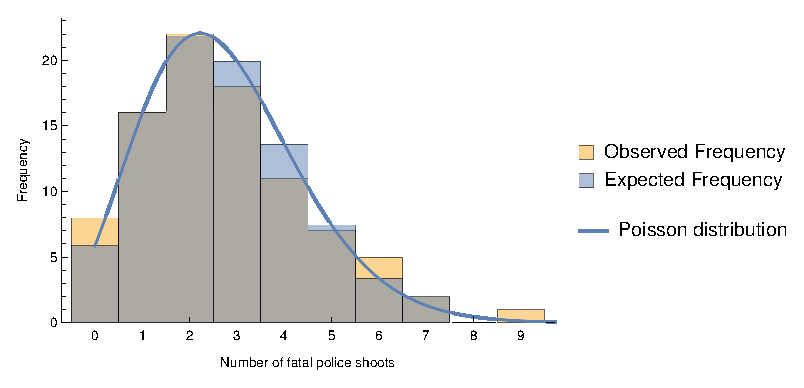
\includegraphics[height=7cm]{q6/q6.eps}
\caption{Observed Frequency $O_i$, Expected Frequency $E_i$ and estimated Poisson distribution versus each number of fatal police shootings data in January - March, 2019.}
\label{fig:q6}
\end{figure}

\newpage

\subsection{Prediction of fatal police shootings in 2019}

\subsubsection{The Nelson prediction interval\cite{KRISHNAMOORTHY20111709}}

Let $X$ be the total counts in a sample of size $n$ from a Poisson distribution with an estimated parameter (mean) $\hat{k}$. Let $Y$
denote the future total counts that can be observed in a sample of size  $m$ from the same Poisson distribution. An estimator of $Y$ is
\begin{equation}
\hat{Y}=m\hat{k}=\frac{mX}{n}
\end{equation}
since $$\frac{\hat{Y}}{m}=\frac{X}{n}=\hat{k}.$$

Then we can find the mean and variance of the linear combination $m\hat{k}-Y$, where $m\hat{k}$ and $Y$ are independent random variables.
\begin{equation}
E[m\hat{k}-\hat{Y}]=E[m\hat{k}]-E[Y]=m\lambda-m\lambda=0
\end{equation}
\begin{equation}
\text{Var}[m\hat{k}-Y]=\text{Var}\left[\frac{m}{n}X-Y\right]=\frac{m^2}{n^2}\text{Var}[X]-\text{Var}[Y]=\frac{m^2}{n^2}n\hat{k}+m\hat{k}=m^2\hat{k}\left(\frac{1}{m}+\frac{1}{n}\right)=m\hat{Y}\left(\frac{1}{m}+\frac{1}{n}\right)
\end{equation}

According to the Central Limit Theorem, if $n$ and $m$ are large enough, \begin{equation}
Z=\frac{m\hat{k}-\hat{Y}-E[m\hat{k}-\hat{Y}]}{\sqrt{\text{Var}[m\hat{k}-Y]}}
\end{equation}
is approximately standard normal, and so the confidence interval length $L$ for a $(1-\alpha)100\%$ confidence interval can be determined by
\begin{align*}
1-\alpha&=P[\hat{Y}-L\leqslant Y\leqslant\hat{Y}+L]\\
&=P\left[\frac{m\hat{k}-\hat{Y}-L}{\sqrt{\text{Var}[m\hat{k}-Y]}}\leqslant0\leqslant\frac{m\hat{k}-\hat{Y}+L}{\sqrt{\text{Var}[m\hat{k}-Y]}}\right]\\
&=P\left[-\frac{L}{\sqrt{\text{Var}[m\hat{k}-Y]}}\leqslant Z\leqslant\frac{L}{\sqrt{\text{Var}[m\hat{k}-Y]}}\right]\\
&=2P\left[0\leqslant Z\leqslant\frac{L}{\sqrt{\text{Var}[m\hat{k}-Y]}}\right]\\
&=1-2P\left[\frac{L}{\sqrt{\text{Var}[m\hat{k}-Y]}}\leqslant Z\leqslant\infty\right].
\end{align*}

Thus we determine $L$ as being the number such that
\begin{equation}
P\left[\frac{L}{\sqrt{\text{Var}[m\hat{k}-Y]}}\leqslant Z\leqslant\infty\right]=\frac{\alpha}{2}.
\end{equation}

But this means that
\begin{equation}
L=z_{\alpha/2}\sqrt{\text{Var}[m\hat{k}-Y]}=z_{\alpha/2}\sqrt{m\hat{Y}\left(\frac{1}{m}+\frac{1}{n}\right)}.
\end{equation}

We get the $(1 - \alpha)100\%$ confidence interval for $Y$,
\begin{equation}\label{eq:q7}
\hat{Y} \pm z_{\alpha / 2} \sqrt{m\hat{Y}\left(\frac{1}{m}+\frac{1}{n}\right)}.
\end{equation}

\subsubsection{Prediction}

The Nelson prediction interval is also valid under the assumption of large sample sizes and an approximate normal distribution of the estimator for $k$ in our cases. \medskip 

Then we can predict the count of fatal police shootings in 2019. First we calculate
$$\hat{Y}=\frac{mX}{n}=\frac{365\cdot3943}{1461}\approx985.075$$
and a 95\% 95\% confidence interval with $z_{\alpha/2}\approx1.96$
$$\hat{Y} \pm z_{\alpha / 2} \sqrt{m\hat{Y}\left(\frac{1}{m}+\frac{1}{n}\right)}\approx(916.304, 1053.85).$$

So our prediction of the fatal police shootings in 2019 is between 916 and 1054. Furthermore, let $m$ be an variable between 1 and 365, we can get an accumulate prediction function
$$f(m)=\frac{mX}{n}$$
and two corresponding prediction confidence bounds
\begin{align*}
f_L(m)&=f(m)-z_{\alpha / 2} \sqrt{mf(m)\left(\frac{1}{m}+\frac{1}{n}\right)},\\
f_R(m)&=f(m)+z_{\alpha / 2} \sqrt{mf(m)\left(\frac{1}{m}+\frac{1}{n}\right)}.
\end{align*}

The functions were plotted in Figure \ref{fig:q7}.
\begin{figure}[!htbp]
\centering
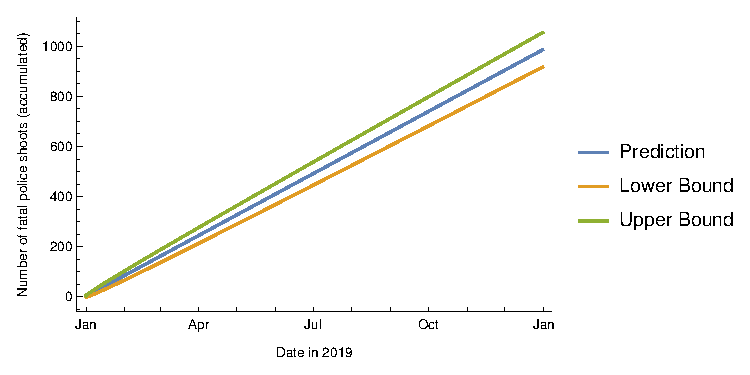
\includegraphics[height=7cm]{q7/q7.eps}
\caption{Predicted fatal police shootings and 95\% confidence bounds in 2019.}
\label{fig:q7}
\end{figure}

With the data for 2019 so far, plotted in Figure \ref{fig:q7-actual}, we can find that most of the actual data falls in the 95\% confidence interval. So we can conclude that our prediction model is appropriate.

\begin{figure}[!htbp]
\centering
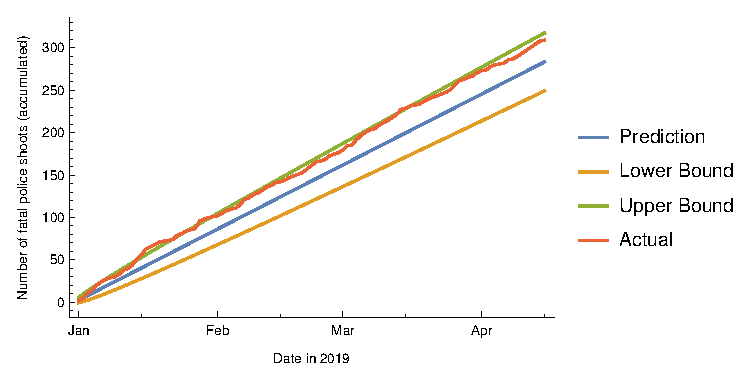
\includegraphics[height=7cm]{q7/q7-actual.eps}
\caption{Predicted and actual fatal police shootings and 95\% confidence bounds in 2019 so far.}
\label{fig:q7-actual}
\end{figure}

\newpage

\section{Conclusion}
In this paper, we look into the pattern of police shootings in US using the data from \textit{Database of Fatal Police Shootings} of the Washington Post.

We find that the occurrence of police shootings in the years 2015-2018 follows a Poisson distribution with parameter $k\approx2.70$. We also get the $95\%$ confidence interval of the parameter $k$ of the four years. We then find that the occurrence of police shootings does not depend on the weekday. At last, We predict that the number of fatal police shootings in 2019 is between 916 and 1054.

Data is powerful if we know how to use it. We can understand the past and predict the future if we know how to obtain and analyze the data.
\newpage

\section{Appendix}

\subsection{Code}

\subsubsection{Overview plot}~

\includegraphics[width=\textwidth]{q2/q2.pdf}

\subsubsection{Distribution between 2015 and 2018}~

\includegraphics[width=\textwidth]{q3/q3-1.pdf}

\includegraphics[width=\textwidth]{q3/q3-2.pdf}

\newpage

\subsubsection{Independence test}~

\includegraphics[width=\textwidth]{q4/q4-1.pdf}

\includegraphics[width=\textwidth]{q4/q4-2.pdf}

\newpage

\subsubsection{Confidence interval of $k$}~

\includegraphics[width=\textwidth]{q5/q5.pdf}

\newpage

\subsubsection{Distribution in early 2019}~

\includegraphics[width=\textwidth]{q6/q6.pdf}

\newpage

\subsubsection{Prediction in 2019}~

\includegraphics[width=\textwidth]{q7/q7.pdf}

\newpage

\bibliography{main} 

\end{document}
